% Minimal LaTeX template
\documentclass[11pt]{article}

% Encoding
\usepackage[utf8]{inputenc}
\usepackage[
  backend=biber,
  style=authoryear,
  giveninits = true,
  uniquename = init,
  natbib
]{biblatex}
\addbibresource{references.bib}
\usepackage{graphicx}
\usepackage{amsmath,amssymb}
\usepackage[T1]{fontenc}
\usepackage[english]{babel}
\usepackage{microtype}
\usepackage{csquotes}   
\usepackage{geometry}
\geometry{margin=2.5cm}
\usepackage{graphicx}
\usepackage{subcaption}
\usepackage{booktabs}
\usepackage{amsmath,amssymb}
\usepackage{siunitx}
\usepackage{hyperref}
\usepackage{cleveref}

\title{Analysis of Style Representation through Gram Matrices}
\author{Antonello Di Rita \\ Bachelor of Science in Artificial Intelligence}
\date{\today}

\begin{document}

\maketitle

\begin{abstract}
\textbf{Aim} — This work aims to determine whether Gram matrices of convolutional feature activations encode \emph{art-historical style} well enough to distinguish movements
such as \emph{Impressionism} and \emph{Baroque} when different distance metrics are applied.\\[2pt]
\textbf{Method} — Gram matrices were computed from five VGG-19 layers for 24 style-labelled paintings in the WikiArt dataset. Similarity between every pair of Gram matrices
was measured using \emph{RMSE}, \emph{Pearson correlation}, and \emph{cosine similarity}.
Differences between intra- and inter-style distances were evaluated by averaging across Gram levels and images.
New images were then synthesized by combining content and style representations extracted with VGG-19 from separate paintings, and their quality was assessed with theLAION Aesthetic Predictor.\\[2pt]
\textbf{Results} — Gram-matrix distances proved to be dominated by global luminance and saturation, yielding minimal separation between conventional styles.
\emph{Pearson correlation} and \emph{cosine similarity} offered slightly better discrimination between styles than \emph{RMSE}.
Overall, Gram matrices alone are a weak descriptor for canonical style classification.\\[2pt]
\end{abstract}


\tableofcontents

\section{Introduction}
\section{Dataset}
\subsection{Source: the \texttt{huggan/wikiart} corpus}
The original \textbf{WikiArt} collection on Hugging~Face\footnote{Dataset card: \url{https://huggingface.co/datasets/huggan/wikiart}} contains \num{81444} digitised
paintings by \num{129} artists annotated with \num{27} art‑historical styles, \num{11} genres,
and \num{129} artist identities. When downloaded as JPEG files, the archive occupies roughly \SI{70}{GB}.
Because the goal is to investigate the discriminative power of Gram matrices rather than to train a classifier,
a deliberately smaller subset is used.

\subsection{Subset construction}
A total of \textbf{100} images were randomly sampled. The sample spans \textbf{21} WikiArt styles; the four most
frequent—\textbf{Baroque}, \textbf{Impressionism}, \textbf{Realism}, and \textbf{Romanticism}—were retained
and each down‑sampled to six images to obtain a perfectly balanced working set of \num{24} paintings.

\subsection{Visual overview of the subset}
Figure~\ref{fig:samples} displays one representative thumbnail for each of the four selected styles.

\begin{figure}[htbp]
    \centering
    \begin{subfigure}[t]{.24\textwidth}
        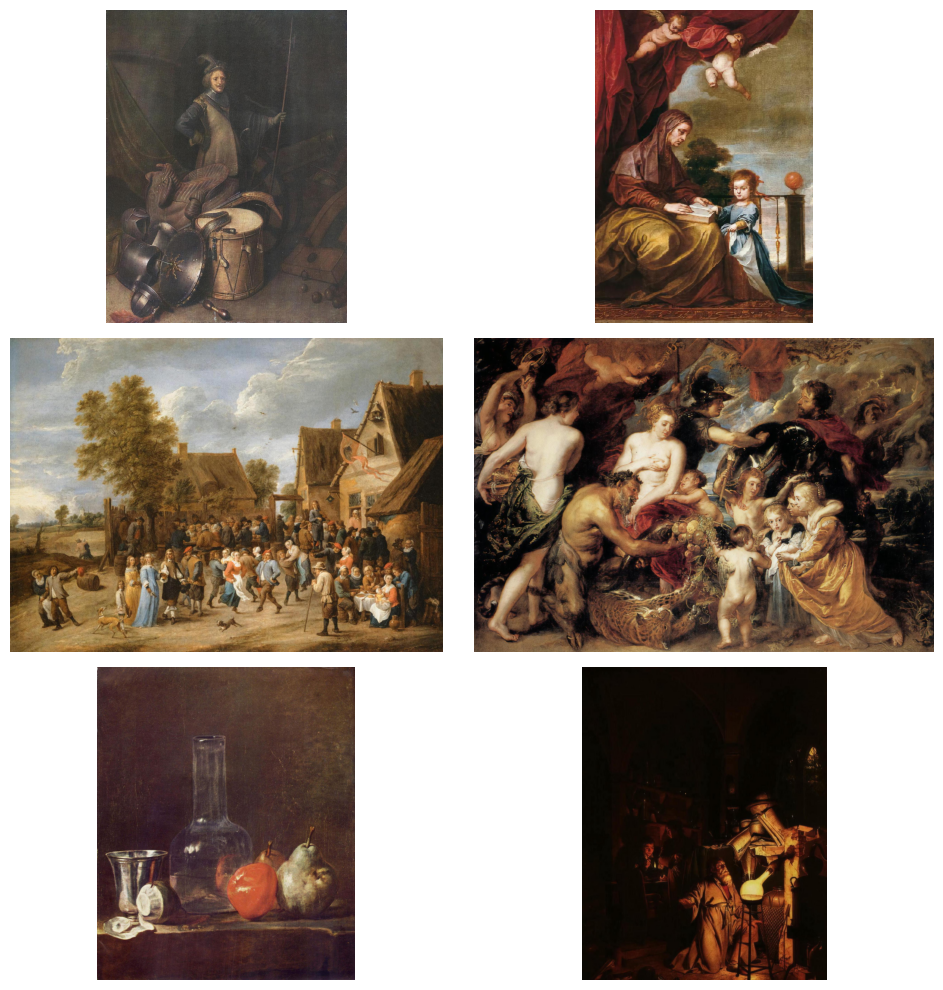
\includegraphics[width=\linewidth]{../figures/Baroque.png}
        \caption{Baroque}
    \end{subfigure}
    \begin{subfigure}[t]{.24\textwidth}
        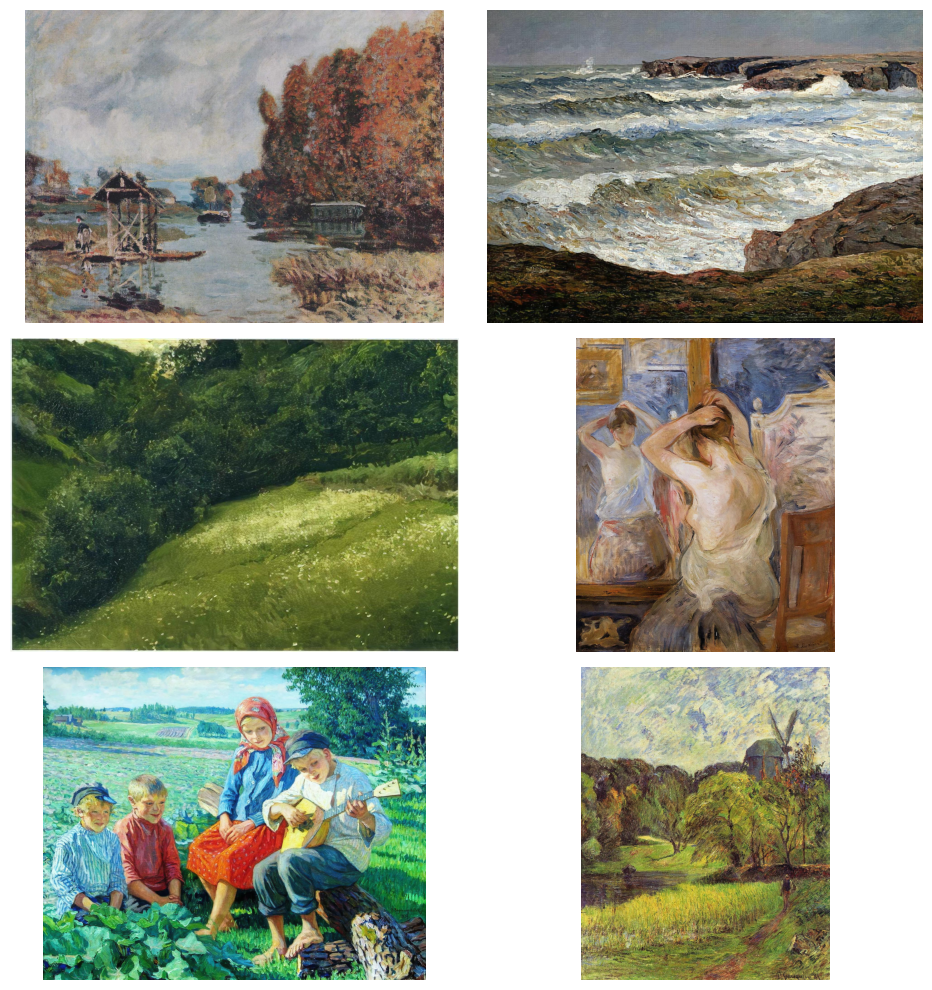
\includegraphics[width=\linewidth]{../figures/Impressionism.png}
        \caption{Impressionism}
    \end{subfigure}
    \begin{subfigure}[t]{.24\textwidth}
        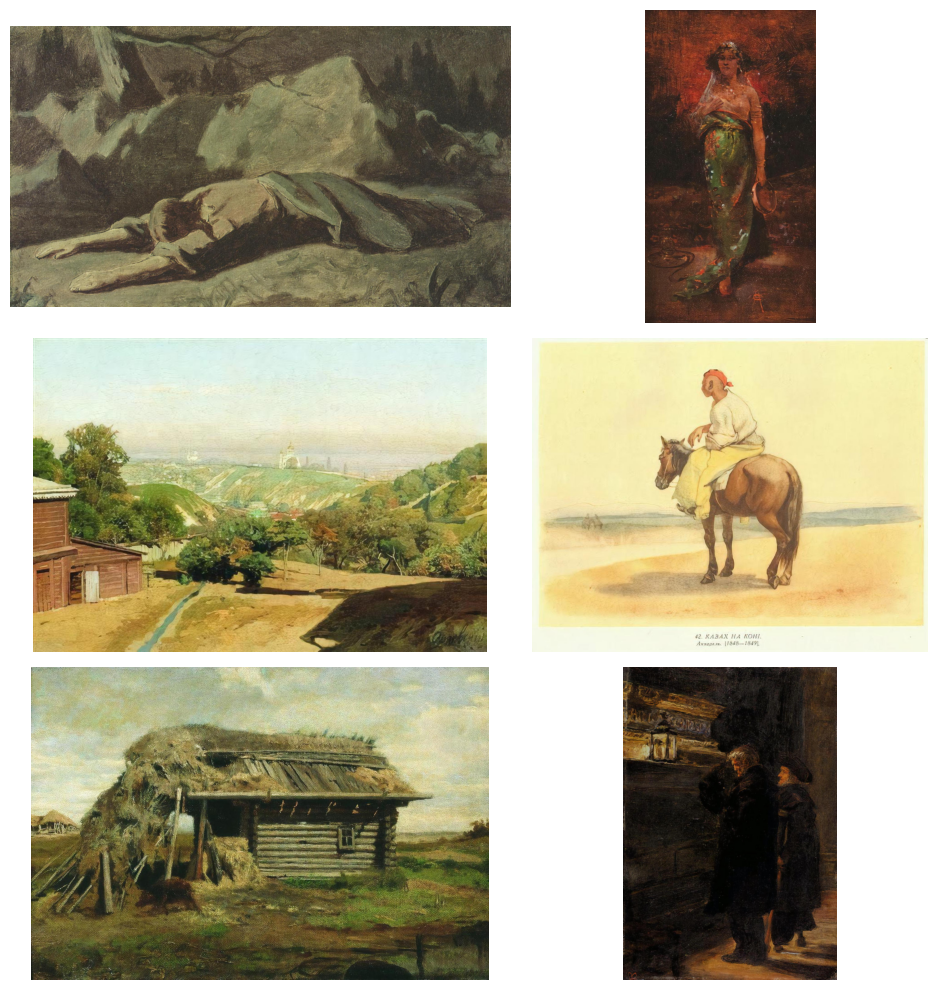
\includegraphics[width=\linewidth]{../figures/Realism.png}
        \caption{Realism}
    \end{subfigure}
    \begin{subfigure}[t]{.24\textwidth}
        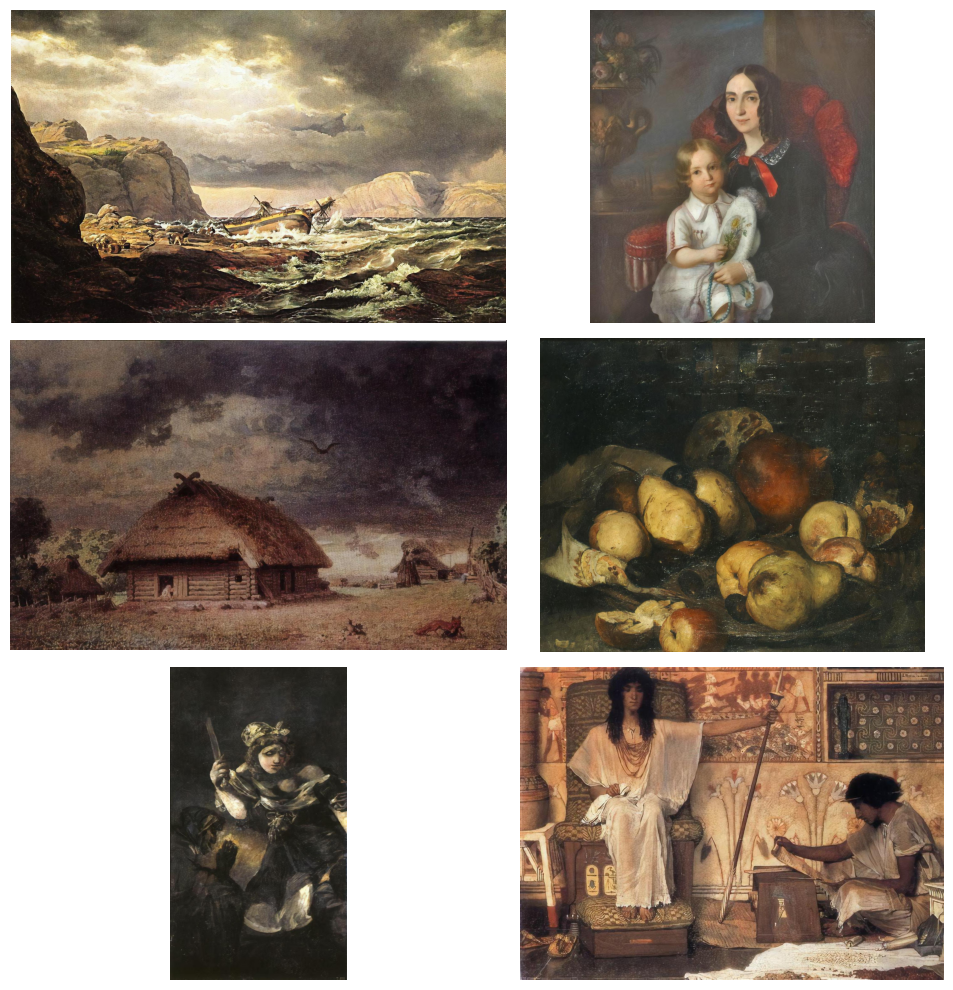
\includegraphics[width=\linewidth]{../figures/Romanticism.png}
        \caption{Romanticism}
    \end{subfigure}
    \caption{Representative paintings for the four art styles retained in the study.}
    \label{fig:samples}
\end{figure}

\section{Methodology}

\subsection{Network backbone}

\subsection{Feature layers and Gram extraction}

\subsection{Pairwise similarity metrics}

\subsubsection{Intra-style experiment}

\subsubsection{Inter-style experiment}

\paragraph{Realism Outlier Experiment}

\subsubsection{Aggregated statistics and visualisation}

\subsection{Image synthesis}

\subsubsection{Content and style extraction}

\subsubsection{Subset Expansion}

\subsubsection{Image quality assessment}

\section{Results and Discussion}

\end{document}